\documentclass[border=10pt]{standalone}
\usepackage{tikz}
\usetikzlibrary{decorations.pathreplacing,arrows.meta}
\definecolor{cwork}{RGB}{72,116,158}
\definecolor{csetup}{RGB}{86,156,104}
\definecolor{crepair}{RGB}{198,86,76}
\definecolor{cpm}{RGB}{222,158,74}
\begin{document}
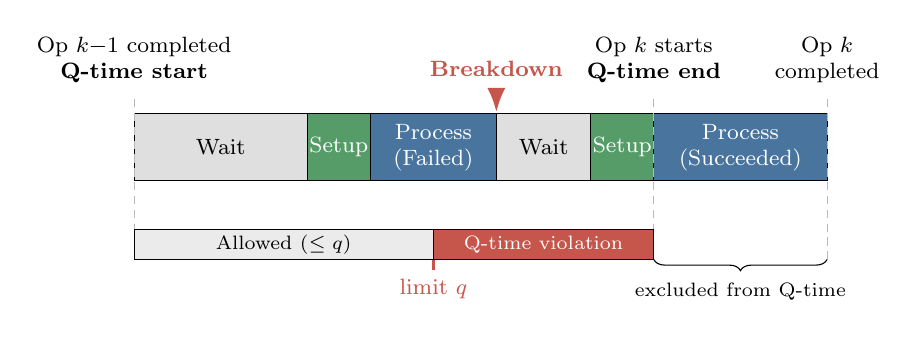
\begin{tikzpicture}[font=\small,>=Latex]
 \def\h{0.85}
 % ---- segment boxes ----
 \foreach \xa/\xb/\c/\tc/\lab in {%
 0/2.2/gray!25/black/Wait, 2.2/3.0/csetup/white/Setup, 3.0/4.6/cwork/white/{Process \\ (Failed)},
   4.6/5.8/gray!25/black/Wait, 5.8/6.6/csetup/white/{Setup}, 6.6/8.8/cwork/white/Process \\ (Succeeded)} {
   \fill[\c](\xa,0)rectangle(\xb,\h); \draw(\xa,0)rectangle(\xb,\h);
   \node[align=center,font=\footnotesize,text=\tc] at ({(\xa+\xb)/2},\h/2){\lab};}
 % ---- start / end guide ticks ----
 \foreach \x in {0,6.6,8.8}\draw[densely dashed,gray!55](\x,-1.0)--(\x,1.1);
 \node[anchor=south,align=center,font=\footnotesize] at (0,1.12){Op $k{-}1$ completed\\\textbf{Q-time start}};
 \node[anchor=south,align=center,font=\footnotesize] at (6.6,1.12){Op $k$ starts\\\textbf{Q-time end}};
 \node[anchor=south,align=center,font=\footnotesize] at (8.8,1.12){Op $k$\\completed};
 % ---- breakdown marker ----
 \draw[crepair,line width=1.3pt,->](4.6,0.98)--(4.6,\h+0.02);
 \node[crepair,anchor=south,font=\footnotesize\bfseries] at (4.6,1.2){Breakdown};
 % ---- budget bar (allowed vs violation) ----
 \def\ya{-1.0}\def\yb{-0.62}
 \fill[black!8](0,\ya)rectangle(3.8,\yb); \draw(0,\ya)rectangle(3.8,\yb);
 \fill[crepair](3.8,\ya)rectangle(6.6,\yb); \draw(3.8,\ya)rectangle(6.6,\yb);
 \node[font=\scriptsize] at (1.9,{(\ya+\yb)/2}){Allowed ($\le q$)};
 \node[font=\scriptsize,text=white] at (5.2,{(\ya+\yb)/2}){Q-time violation};
 % q boundary tick (below the bar)
 \draw[crepair,line width=0.9pt](3.8,\ya)--(3.8,\ya-0.13);
 \node[crepair,anchor=north,font=\footnotesize] at (3.8,\ya-0.13){limit $q$};
 % ---- 'excluded' brace under normal process ----
 \draw[decorate,decoration={brace,amplitude=4pt,mirror}](6.6,\ya)--(8.8,\ya)
   node[midway,below=5pt,font=\scriptsize,align=center]{excluded from Q-time};
\end{tikzpicture}
\end{document}
